\chapter{Einführung}
\label{cha:1}

\section{Was ist Wärmeübertragung}

Die Beobachtung der Naturvorgänge, die mit dem Transport der Wärme zu tun haben, hat zu einer Feststellung geführt. Und zwar, falls ein Medium zwei Gebiete mit unterschiedlichen Temperaturen besitzt, bewegt sich die Wärme immer aus dem Gebiet mit der höheren Temperatur in das, wo eine niedrigere Temperatur herrscht. Dieser Vorgang der Wärmeübertragung kann auf drei Arten geschehen, durch sogenannte Wärmeleitung, durch Wärmekonvektion und durch Wärmestrahlung. Im folgendem wollen wir diese Begrifflichkeiten zuerst klären.

\subsection{Wärmeleitung}

Man stelle sich vor, wie ein Metallstab an einem Ende aufgeheizt wird. Nach einiger Zeit würde man an dem anderem Ende eine Temperaturerhöhung messen können. Im Umkehrschluss hieße es, dass die Wärme von dem Stabende, wo eine Wärmequelle angelegt wurde, zu dem anderem gewandert ist. Eine physikalische Erklärung dafür könnte so lauten, die Atome, wo eine Wärmequelle angelegt ist, fangen an stärker zu schwingen, also bekommen mehr Energie. Durch die Gitterstruktur im Metall regen die schon stärker schwingende Atome ihre Nachbarn an und so weiter, bis die Atome an dem anderem Ende auch stärker schwingen. Somit wird die Wärmeenergie in Form schwingender Atome durch einen Festkörper transportiert, in solchen Fällen spricht man von \textit{Wärmeleitung}.

\subsection{Wärmekonvektion}

Bei der \textit{Konvektion} handelt es sich um Transport der Stoffmengen. Dieser Prozess findet in festen, flüssigen und gasförmigen Materialzuständen statt. Zum Beispiel bei Flüssigkeiten und Gasen tritt eine Ausgleichsströmung durch den Dichteunterschied zwischen warmen und kühleren Gebieten auf. In solchen Fällen sind die wärmeren Gebiete spezifisch leichter und steigen in die Höhe, wo sie sich dann abkühlen. Der beschriebene Verlauf ist ein Fall für sogenannte \textit{freie Konvektion}. Eine \textit{erzwungene Konvektion} liegt dann vor, wenn eine äußere Einwirkung dem System hinzugefügt wird. Hierfür könnte eine Vulkaneruption als Beispiel dienen. 

\subsection{Wärmestrahlung}

\begin{figure}[!h]
	\centering
	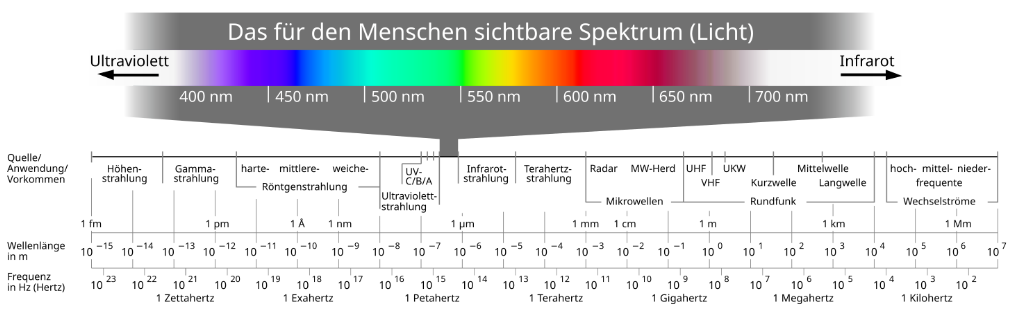
\includegraphics[width=\textwidth]{em_spektrum}
	\caption{Das Spektrum der elektromagnetischen Strahlung. Quelle: \href{https://de.wikipedia.org/wiki/Elektromagnetisches_Spektrum}{Wikipedia}.}
	\label{fig:1.1.3_1}
\end{figure}

Im Vakuum, da wo keine Materie vorhanden ist, kann die Wärmeübertragung weder durch Wärmeleitung noch durch Konvektion stattfinden. Nehmen wir ein Beispiel der Wärmeübertragung von der Sonne zur Erde an. Trotzt der Tatsache, dass der Raum zwischen der Erde und Sonne (fast) leer von Materie ist, findet die Wärmeübertragung von der Sonne auf die Erde statt. Es ist die \textit{Wärmestrahlung }, die für die Energieübertragung sorgt. Im Allgemeinen werden solche Prozesse durch das Konzept der elektromagnetischen Strahlung erklärt. Fakt ist, dass die elektromagnetische Strahlung kein Medium braucht um sich im Raum auszubreiten. Strahlung an sich kann mittels Wellen mathematisch beschrieben werden. Wellen schwingen, alles was schwingt hat eine Frequenz und kann daher in einem Frequenzspektrum eingeordnet werden. So ist die Wärmestrahlung nur ein Teil des gesamten elektromagnetischen Spektrums, wobei die UV-Strahlung, das sichtbare Spektrum und die Infrarot-Strahlung die Wärmestrahlung ausmachen (Abb.\ref{fig:1.1.3_1}). Tritt die Wärmestrahlung auf Materie, so wird sie absorbiert, wodurch sich die Materie aufwärmt oder gar erhitzt.

\section{Definition des Vorhabens}

\subsection{Das Problem}

Die vorangegangenen Überlegungen werden unten im Text herangezogen, um die theoretische Herangehensweise zum Problem der Wärmeausbreitung in Stoffen bereitzustellen ... bla bla ... was wird gemacht:

\begin{enumerate}
	\item Überlegungen, die aus physikalischen Gegebenheiten auf eine Gleichung Führen, im Kapitel \ref{cha:2}.
	\item Gleichung benennen, als Wärmegleichung, ev. Kapitel so und so.
	\item Mögliche Problemstellungen benennen, direkte und inverse ..., ev. Kapitel so und so
	\item Das Vorhaben benennen. Mit NN inverses Problem lösen, bla bla
	\item Die Struktur des Vorhabens schildern: FEM -> Lösung -> einige Werte der Lösung als Input für NN, , ev. Kapitel so und so
	\item Vergleich der Ergebnisse, ev. Kapitel so und so
\end{enumerate}
 Bla Bla ... somit ist das Ziel der vorliegenden Arbeit festgelegt worden
